\documentclass{report}
\usepackage{color}
\usepackage[utf8x]{inputenc}
\usepackage[T1]{fontenc}      % caractères français
\usepackage{geometry}         % marges
\usepackage[francais]{babel}  % langue
\usepackage{graphicx} 
\usepackage{wrapfig}
\usepackage{listingsutf8}
\usepackage[final]{pdfpages} 
\usepackage{float}

\usepackage{amsmath}
\usepackage{enumitem}     % images
\usepackage{verbatim}         % texte préformaté
\title{\LARGE Implémentation d'un outil de veille concurrentielle concernant des articles de loisirs sportifs}      % renseigne le titre
\author{Clément BALESTRAT - Nicolas KERMARC - Yann PRAVOSSOUDOVITCH}
          
\pagestyle{headings}          % affiche un rappel discret (en haut à gauche)
                         % de la partie dans laquel on se situe
                         
\makeatletter
\def\thetitle{\@title}
\def\theauthor{\large\@author}
\def\thedate{\@date}
\makeatother
\definecolor{light-gray}{gray}{0.95}
\lstset{backgroundcolor=\color{light-gray}, inputencoding=utf8/latin1}
\begin{document}
\begin{titlepage}


\includegraphics[scale=0.1]{logo.jpg} 

\centering
\vfill
{\Huge\bfseries \thetitle}
\vskip 1cm
{\Large \theauthor}
\hspace{10.5cm}
\vskip 0.25cm
\Large Rapport de synthèse du Projet Industriel de Fin d'Etudes\\
\Large Département Informatique et Gestion
\vskip 0.25cm
\Large 25 janvier 2013
\vskip 0.5cm
\vfill
\large Tuteur: Anne-Laure De Lauzun
\hspace{2cm}
\large Demandeur: Sébastien BERNIS
\end{titlepage}



\renewcommand{\contentsname}{Sommaire}
 


\tableofcontents

\chapter{Introduction}

\paragraph{}

Dans le cadre de nos études, un Projet Industriel de Fin d'Etudes (PIFE) est à réaliser par groupe d'étudiants. Ce projet, étalé sur une période de deux mois a pour but de faire travailler les étudiants sur un sujet pour une entreprise, tout en restant dans le cadre des études. Ce rapport a donc pour but de faire une synthèse de notre travail durant cette période.

\paragraph{}

Dans une première partie nous verrons donc le contexte de ce projet, avec une brève présentation du demandeur ainsi qu'une description de la demande initiale. \\Puis, dans une seconde partie, notre démarche ainsi que notre organisation utilisées pour mener à bien notre travail seront décrites. \\La partie suivante traitera notre travail effectué. Les résultats intermédiaires et finaux, mais aussi les problèmes techniques seront ici détaillés. \\Enfin une conclusion viendra clôturer ce rapport, avec un bref récapitulatif sur les tenants et les aboutissants de ce projet, mais aussi ce que ce dernier a apporté au groupe et à l'entreprise.
\chapter{Le contexte}

\section{Sébastien BERNIS}

\paragraph{}

Nous avons choisi d'effectuer ce projet industriel pour la société \textit{BERNIS Informatique}, représentée par Sébastien Bernis.
Actuellement employé chez \textit{La Palanquée}, magasin de produits concernant la plongée sous marine à Palavas-les-Flots, Sébastien Bernis a notamment pour tâche la gestion du site internet de l'entreprise, proposant une plateforme de e-commerce.
\newline
Ayant l'habitude de surveiller les articles chez les concurrents, ce dernier s'est rendu compte que les sites de comparaison de prix n'étaient pas des plus justes, car ils auraient la fâcheuse tendance à baser leur affichage en fonction des sociétés qui payent le plus, et non en fonction des prix réels. Il a donc eu pour idée la création d'une véritable plateforme de comparaison de prix en temps réel. Ce service serait proposé uniquement aux professionnels, qui, à n'importe quel moment de la journée pourraient consulter les prix de leurs concurrents directs.



\section{Notre mission}

\paragraph{}

Nous avons donc eu pour mission le développement de ce module de comparaison de prix. L'utilisateur se connectera sur le site et accèdera directement à une page principale avec d'un côté ses prix à lui, et d'un autre les prix de ses concurrents. Il sera donc important de mettre en valeur les prix étant moins chers ailleurs, afin que ce dernier puisse s'en apercevoir rapidement.

\paragraph{}

Deux points semble être ici relativement importants: la bonne récupération des prix et l'afficage de ces derniers en temps réel. 
\\Un identifiant unique pour chaque article n'étant certainement pas présent à tous les moments, il sera donc important d'essayer de faire correspondre au mieux les désignations et modèles de ces derniers. Il arrive que les prix puissent varier plusieurs fois dans la journée. Il est donc primordial d'afficher les bons prix à l'utilisateur. Notre algorithme devra par conséquent être des plus efficace, afin de proposer une mise à jour des tarifs très rapidement.\\
Il est bien évidemment nécessaire de traiter uniquement les articles que l'utilisateur possède. Ce dernier n'aura pas besoin de consulter des prix pour des produits qu'il ne vend pas.
\\
Pour l'instant notre projet a été limité à quelques sites d'articles de plongée comme \textit{scubastore.com}, \textit{palanquee.com}, \textit{bubble-diving.com}, \textit{vieuxplongeur.com} et \textit{scubaland.com}.   

\paragraph{}

Il faut bien comprendre que mis à part ces détails, aucune indication supplémentaire nous a été donnée. C'est d'ailleurs pour ça que ce projet nous a séduit au départ. En effet, il nous a donné la possibilité de partir de rien pour espérer arriver à un rendu exploitable. Un long travail de conception, d'implémentation et de déploiement nous attendait. Bien évidemment pour chaque choix conceptuel nous avons pu en parler directement avec M. Bernis qui s'est porté volontaire, dès le départ, à nous rencontrer chaque semaine afin de faire le point sur nos avancements. Nous avons eu cependant une totale liberté de mouvement vis à vis des choix technologiques.

\paragraph{}
Notre premier travail a donc été la rédaction de la lettre de mission, afin de clarifier tous les points au sujet de ce que voulait le demandeur.
De ce fait, un listing récapitulatif des fonctions de l'application a été établi:

\begin{itemize}
\item Récupération des articles et des prix sur les sites précédemments cités à l'aide de scripts automatiques dits \textit{robots}.
\item Développement d'une interface utilisateur relativement basique, mais claire.
\item Gérer l'affichage des articles que vend l'utilisateur et y associer les prix des concurrents, tout en mettant en valeur ceux qui sont inférieurs.
\item Implémenter un système de mise à jour des prix et des articles afin que l'utilisateur puisse toujours avoir des données correctes.
\end{itemize}

\paragraph{}
C'est donc à partir de cette liste que nous avons pu démarrer notre travail.

\chapter{Organisation et démarche}

\section{Découpage des tâches et établissement des rôles}
Notre premier travail fût l'analyse des différentes tâches qui allaient composer ce projet. Nous avons pu très vite distinguer plusieurs axes de réflexion et de travail:

\begin{itemize}
\item L'étude de la structure des sites web concernés, afin de voir comment y récupérer les données.
\item La réflexion sur le stockage de ces données. Quel type de base de données ? Quelle(s) structure(s) ? Quel(s) modèle(s)
\item Le choix d'un rendu visuel. Avoir quelque chose de clair, ergonomique et esthétique qui puisse intéragir avec la base de données.
\end{itemize}

\paragraph{}
Nous avons donc pu, dans un premier temps, définir les rôles de chacun. Nicolas Kermarc serait responsable du rendu visuel (\textit{front-end}), Clément Balestrat de la collecte des données sur chacun des sites et Yann Pravossoudovitch responsable de la base de données. \\Pourquoi avoir effectué ce découpage par rôle ? \\Tout simplement parce que nous avons trouvé judicieux le choix de se spécialiser chacun dans un domaine bien précis du projet afin d'être le plus compétent possible, au lieu de "toucher à tout" ce qui au final aurait pu provoquer une perte de temps et un cafouillage général.\\
Ainsi, le travail de Clément serait complémentaire à celui de Yann puisque ce dernier aurait besoin de toutes ces données pour les stocker, et c'est ce stockage qui allait être utile à Nicolas pour pouvoir gérer l'interface utilisateur.\\
Pour ce qui est de la conception générale du projet, il est bien évident qu'un travail d'équipe a eu lieu afin de pouvoir réfléchir tous ensemble et se mettre d'accord sur une idée finale.

\section{La gestion de projet}

\paragraph{}

Ce projet nous a très vite paru lourd en matière de charge de travail. En effet, avec deux mois pour une conception, un développement et un déploiement, le tout accompagné d'une rédaction de rapport de synthèse et technique, il fallait trouver une organisation optimale dans le temps. Après avoir établi le nombre de jours/homme nécessaire au bon déroulement de ce projet, nous avons décidé d'utiliser un diagramme de Gantt afin d'avoir un planning à suivre.

\begin{figure}[H]
\begin{center}
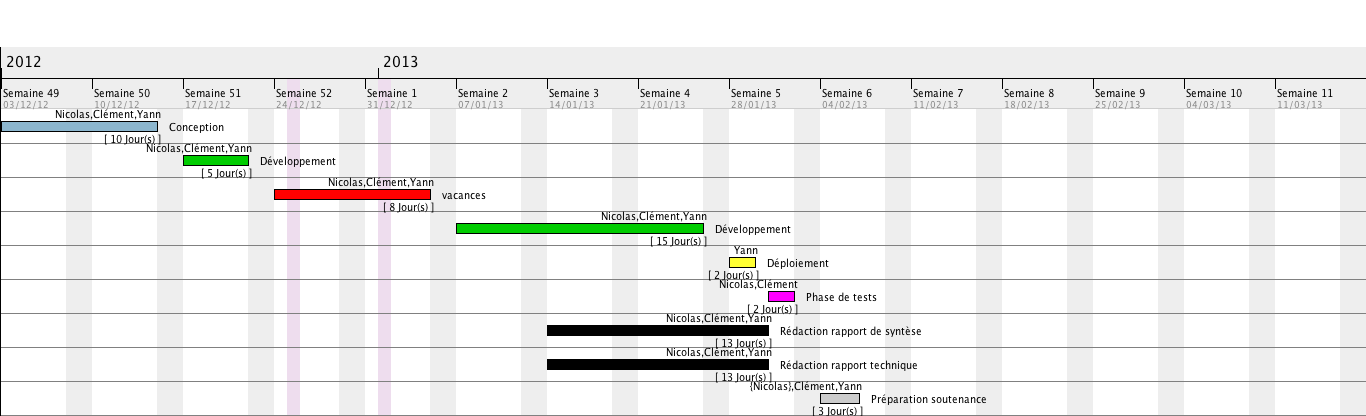
\includegraphics[scale=0.4, angle=90]{diagramme.png}
\caption{\textit{Diagramme de Gantt}}
\end{center}
\end{figure}

\paragraph{}
Comme on peut le voir sur la figure 3.1, les tâches suivantes ont été programmées dans le planning:
\begin{itemize}
\item Conception (10 jours)
\item Développement (20 jours)
\item Rédaction du rapport de synthèse et du rapport technique (13 jours)
\item Déploiement de l'application (2 jours)
\item Phase de tests (2 jours)
\item Préparation de la soutenance (3 jours)
\end{itemize}


\paragraph{}
Plusieurs tâches ont été placées en même temps, comme le développement et la rédaction des rapports. C'est tout simplement qu'un roulement a été plannifié. En effet, à partir du 14 janvier, deux auront pour tâche le développement pendant qu'un autre s'occupera du rapport. Ce roulement est journalier mais peut être allongé pour des raisons particulières (une partie à finir de rédiger pour la personne concernée par exemple). \\

Nous avons jugé que deux personnes étaient utiles pour la rédaction du rapport de synthèse (Clément et Nicolas), et trois personnes pour le rapport technique. Etant donné que chacun aura une mission technique relativement différente durant le projet, il nous a donc semblé normal que chacun détaille sa partie au mieux dans le rapport technique.\\

Pour finir, Yann sera chargé de la partie déploiement tandis que Clément et Nicolas s'occuperont des tests finaux. Un créneau de trois jours à également été réservé afin de pouvoir se préparer pour la soutenance du projet.

\section{Nos outils}
Les choix technologiques ont été établis très rapidement: 
\begin{itemize}
\item PHP pour la partie récupération de données sur les sites de plongée
\item MongoDB pour la gestion de la base de données
\item Node.js pour le front-end
\end{itemize}

\paragraph{}
Pourquoi ces technologies et pas d'autres ? Le PHP est un langage web énormément utilisé et est réputé pour sa rapidité de traitement. Ayant une grosse communauté de développeurs, il possède tout un arsenal de librairies qui va nous servir à récolter très facilement les données sur les sites. \\MongoDB est un Système de Gestion de Base de Données (SGBD) scalable, à hautes performances et open source. Nous avions déjà eu l'occasion de l'utiliser lors du précédent projet industriel chez \textit{Deegr.com} et sa facilité d'utilisation nous avait charmés.\\Enfin, Node.js car il permet de faire du JavaScript côté serveur, et est réputé pour ses bonnes performances.\\
Une description plus détaillée sur ces technologies est présente dans le rapport technique.

\paragraph{}
En ce qui concerne les outils de travail collaboratif, nous avons utilisé Github, qui est un logiciel de versions décentralisées. Il permet à un groupe de développeurs de travailler sur un même projet sans avoir à s'envoyer les sources à chaque fois qu'elles ont été mises à jour. En effet, un simple \textit{push} permet à une membre de l'équipe de mettre à jour ses changements sur le serveur Git, et \textit{pull} pour récupérer la dernière version du projet sur son poste.\\
Cet outil est indispensable pour le bon déroulement d'un projet en équipe.

\begin{figure}[H]
\begin{center}

\includegraphics[scale=0.4]{git.png}
\caption{\textit{Github}}
\end{center}
\end{figure}

\paragraph{}
Enfin, M. Bernis a eu l'idée de nous louer un serveur dédié chez OVH afin de pouvoir héberger notre projet, mais aussi dans le but de gagner en performance lors de l'exécution des robots ou de l'algorithme de matching, cette dernière pouvant être fastidieuse et gourmande en ressources, poussant souvent nos Macbook Pro dans leurs derniers retranchements.

\begin{figure}[H]
\begin{center}

\includegraphics[scale=1.2]{ovh.jpg}
\caption{\textit{OVH}}
\end{center}
\end{figure}

\chapter{La conception}

\section{Les modèles}

\section{Idées supplémentaires}

\section{Problèmes rencontrés}

\section{Orientation vers une nouvelle solution}

\section{Maquettes}

\chapter{Le développement}

\section{Nos méthodes}

\section{Le résultat final}

\section{Problèmes techniques rencontrés}


\chapter{Conclusion}






\end{document}
